%!TEX root = ../../ThesisRomainBrault.tex

\section{Operator-valued functions and integration}

\section{About concentration inequalities}

\section{ORFF Engineering}
\section{Learning with semi-supervision}
We present here an extension of \cref{ch:learning
operator-valued_random_fourier_features} to semi-supervised learning with
\acs{ORFF} in the framework of~\citet{minh2016unifying}. This framework
includes Vector-valued Manifold
Regularization~\citep{belkin2006manifold,Brouard2011,minh2013unifying} and
Co-regularized Multi-view
Learning~\citep{brefeld2006efficient,sindhwani2008rkhs,rosenberg2009kernel,
sun2011multi}.

\subsection{Representer theorem and feature equivalence}
We suppose that we are given a training sample
$\seq{u}=(x_i)_{i=N}^{N+U}\in\mathcal{X}^U$ of unlabeled exemples. We note
$\seq{z}\in\left(\mathcal{X}\times\mathcal{Y}\right)^N\times\mathcal{X}^U$ the
sequence $\seq{z}=\seq{s}\seq{u}$ concatenating both labeled ($\seq{s}$) and
unlabeled ($\seq{u}$) training examples.
\begin{theorem}[Representer theorem, \citet{minh2016unifying}]
    \label{th:representer_semi}
    Let $K$ be a $\mathcal{U}$-Mercer \acl{OVK} and $\mathcal{H}_K$ its
    corresponding $\mathcal{U}$-Reproducing Kernel Hilbert space.
    \paragraph{}
    Let $V:\mathcal{U}\to\mathcal{Y}$ be a bounded linear operator and let
    $c:\mathcal{Y}\times\mathcal{Y}\to\overline{\mathbb{R}}$ be a cost function
    such that $L(x, f, y)=c(Vf(x), y)$ is a proper convex lower semi-continuous
    function in $f$ for all $x\in\mathcal{X}$ and all $y\in\mathcal{Y}$.
    \paragraph{}
    Eventually let $\lambda_K\in\mathbb{R}_{>0}$ and $\lambda_M \in
    \mathbb{R}_+$ be two regularization hyperparameters and
    $(M_{ik})_{i,k=1}^{N+U}$ be a sequence of data dependent bounded linear
    operators in $\mathcal{L}(\mathcal{U})$, such that
    \begin{dmath*}
        \sum_{i,j=1}^{N+U} \inner{u_i, M_{ik}u_k} \ge 0 \condition{$\forall
        (u_i)_{i=1}^{N+U}\in\mathcal{U}^{N+U}$ and $M_{ik}=M_{ki}^*$}.
    \end{dmath*}
    The solution $f_{\seq{z}}\in\mathcal{H}_K$ of the regularized optimization
    problem
    \begin{dmath}
        f_{\seq{z}} = \argmin_{f\in\mathcal{H}_K}
        \frac{1}{N}\displaystyle\sum_{i=1}^N c(Vf(x_i), y_i) +
        \frac{\lambda_K}{2}\norm{f}^2_{K} \\ +
        \frac{\lambda_M}{2}\sum_{i,k=1}^{N+U}\inner{f(x_i),
        M_{ik}f(x_k)}_{\mathcal{U}} \label{eq:learning_rkhs_gen_semi}
    \end{dmath}
    has the form $f_{\seq{z}}=\sum_{j=1}^{N+U}K(\cdot,x_j)u_{\seq{z},j}$ where
    $u_{\seq{z},j}\in\mathcal{U}$ and
    \begin{dmath}
        \label{eq:argmin_u_semi} u_{\seq{z}} =
        \argmin_{u\in\Vect_{i=1}^{N+U}\mathcal{U}}\frac{1}{N}
        \displaystyle\sum_{i=1}^N c\left(V\sum_{k=1}^{N+U}K(x_i,x_j)u_j,
        y_i\right) + \frac{\lambda_K}{2}\sum_{k=1}^{N+U}u_i^\adjoint
        K(x_i,x_k)u_k \\ + \frac{\lambda_M}{2}\sum_{i,k=1}^{N+U}
        \inner*{\sum_{j=1}^{N+U}K(x_i,x_j)u_j,
        M_{ik}\sum_{j=1}^{N+U}K(x_k,x_j)u_j}_{\mathcal{U}}.
    \end{dmath}
\end{theorem}
We present here the proof of the formulation proposed
by~\citet{minh2016unifying}. In the mean time we clarify some elements of the
proof. Indeed the existence of a global minimizer is not trivial and we must
invoke the Mazur-Schauder theorem. Moreover the coercivity of the objective
function required by the Mazur-Schauder theorem is not obvious when we do not
require the cost function to take only positive values. However a corollary of
Hahn-Banach theorem linking strong convexity to coercivity gives the solution.
\begin{proof}
    Since $f(x)=K_x^*f$ (see \cref{eq:reproducing_prop}), the optimization
    problem reads
    \begin{dmath*}
        f_{\seq{z}} = \argmin_{f\in\mathcal{H}_K}
        \frac{1}{N}\displaystyle\sum_{i=1}^N c(VK_{x_i}^\adjoint f, y_i) +
        \frac{\lambda_K}{2}\norm{f}^2_{K} \\ +
        \frac{\lambda_M}{2}\sum_{i,k=1}^{N+U}\inner{K_{x_i}^\adjoint f,
        M_{ik}K_{x_k}^\adjoint f}_{\mathcal{U}}
    \end{dmath*}
    Let $W_{V,\seq{s}}:\mathcal{H}_K\to\Vect_{i=1}^N\mathcal{Y}$ be the 
    restriction linear operator defined as
    \begin{dmath*}
        W_{V,\seq{s}}f = \Vect_{i=1}^N VK_{x_i}^\adjoint f,
    \end{dmath*}
    with $VK_{x_i}^\adjoint:\mathcal{H}_K\to\mathcal{Y}$ and
    $K_{x_i}V^\adjoint:\mathcal{Y}\to\mathcal{H}_K$. Let
    $Y=\vect_{i=1}^Ny_i\in\mathcal{Y}^N$. We have
    \begin{dmath*}
        \inner{Y,W_{V,\seq{s}}f}_{\Vect_{i=1}^N\mathcal{Y}} =
        \sum_{i=1}^N\inner{y_i, VK_{x_i}^\adjoint f}_{\mathcal{Y}}
        \hiderel{=}\sum_{i=1}^N\inner{K_{x_i}V^\adjoint y_i,
        f}_{\mathcal{H}_K}.
    \end{dmath*}
    Thus the adjoint operator $W_{V,\seq{s}}^\adjoint :
    \Vect_{i=1}^N\mathcal{Y}\to\mathcal{H}_K$ is
    \begin{dmath*}
        W_{V,\seq{s}}^\adjoint Y=\sum_{i=1}^NK_{x_i}V^\adjoint y_i,
    \end{dmath*}
    and the operator $W_{V,\seq{s}}^* W_{V,\seq{s}} : \mathcal{H}_K \to
    \mathcal{H}_K$ is
    \begin{dmath*}
        W_{V,\seq{s}}^\adjoint W_{V,\seq{s}}f = \sum_{i=1}^NK_{x_i}V^\adjoint
        VK_{x_i}^\adjoint f
    \end{dmath*}
    where $V^\adjoint V\in\mathcal{L}(\mathcal{U})$. Let
    \begin{dmath*}
        J_{\lambda_K}(f) = \underbrace{\frac{1}{N}\displaystyle\sum_{i=1}^N
        c(Vf(x_i), y_i)}_{=J_c} + \frac{\lambda_K}{2}\norm{f}^2_{K} \\ +
        \underbrace{\frac{\lambda_M}{2}\sum_{i,k=1}^{N+U}\inner{f(x_i),
        M_{ik}f(x_k)}_{\mathcal{U}}}_{=J_M}
    \end{dmath*}
    Since $c$ is proper, lower semi-continuous and
    convex by assumption, thus the term $J_c$ is also proper, lower
    semi-continuous and convex. Moreover the term $J_M$ is always positive for
    any $f\in\mathcal{H}_K$ and $\frac{\lambda_K}{2}\norm{f}^2_{K}$ is strongly
    convex.  Thus $J_{\lambda_K}$ is strongly convex. Apply
    \cref{lm:strongly_convex_is_coercive} to obtain the coercivity of
    $J_{\lambda_K}$, and then \cref{cor:unique_minimizer} to show that
    $J_{\lambda_K}$ has a unique minimizer and is attained. Then let
    \begin{dmath*}
        \mathcal{H}_{K, \seq{z}}=\Set{\sum_{j=1}^{N+U}K_{x_j}u_j| \forall
        (u_i)_{i=1}^{N+U} \in\mathcal{U}^{N+U}}.
    \end{dmath*}
    For $f\in\mathcal{H}_{K, \seq{z}}^\perp$, the operator
    $W_{V,\seq{s}}$ satisfies
    \begin{dmath*}
        \inner{Y, W_{V,\seq{s}}f}_{\Vect_{i=1}^N\mathcal{Y}} =
        \inner{\underbrace{f}_{\in\mathcal{H}_{K, \seq{z}}^\perp},
        \underbrace{\sum_{i=1}^{N+U}K_{x_i}V^\adjoint y_i}_{\in\mathcal{H}_{K,
        \seq{z}}}}_{\mathcal{H}_K} \hiderel{=} 0
    \end{dmath*}
    for all sequences $(y_i)_{i=1}^N$, since $V^\adjoint y_i\in\mathcal{U}$.
    Hence,
    \begin{dmath}
        \label{eq:null1_semi} (Vf(x_i))_{i=1}^{N}=0
    \end{dmath}
    In the same way,
    \begin{dmath*}
        \sum_{i=1}^{N+U}\inner{K_{x_i}^* f, u_i}_{\mathcal{U}} \hiderel{=}
        \inner{\underbrace{f}_{\in\mathcal{H}_{K, \seq{z}}^\perp},
        \underbrace{\sum_{j=1}^{N+U}K_{x_j}u_j}_{\in\mathcal{H}_{K,
        \seq{z}}}}_{\mathcal{H}_K} \hiderel{=} 0.
    \end{dmath*}
    for all sequences $(u_i)_{i=1}^{N+U}\in\mathcal{U}^{N+U}$. As a result,
    \begin{dmath}
        \label{eq:null2_semi} (f(x_i))_{i=1}^{U+N}=0.
    \end{dmath}
    Now for an arbitrary $f\in\mathcal{H_K}$, consider the orthogonal
    decomposition $f = f^{\perp} + f^{\parallel}$, where $f^{\perp} \in
    \mathcal{H}_{K, \seq{z}}^\perp$ and $f^{\parallel} \in \mathcal{H}_{K,
    \seq{z}}$. Then since $\norm{f^{\perp} + f^{\parallel}}_{\mathcal{H}_K}^2
    =\norm{f^{\perp}}_{\mathcal{H}_K}^2 +
    \norm{f^{\parallel}}_{\mathcal{H}_K}^2$, \cref{eq:null1_semi} and
    \cref{eq:null2_semi} shows that if $\lambda_K > 0$, clearly then
    \begin{dmath*}
        J_{\lambda_K}(f)=J_{\lambda_K}\left(f^{\perp}+f^{\parallel}\right)
        \hiderel{\ge} J_{\lambda_K}\left(f^{\parallel}\right)
    \end{dmath*}
    The last inequality holds only when $\norm{f^{\perp}}_{\mathcal{H}_K}=0$,
    that is when $f^{\perp}=0$. As a result since the minimizer of
    $J_{\lambda_K}$is unique and attained, it must lies in $\mathcal{H}_{K,
    \seq{z}}$.
\end{proof}

\begin{theorem}[Feature equivalence]
    \label{th:orff_representer_semi} Let $\tildeK{\omega}$ be an \acl{OVK} such
    that for all $x$, $z\in\mathcal{X}$, $\tildePhi{\omega}(x)^\adjoint
    \tildePhi{\omega}(z) = \widetilde{K}(x,z)$ where $\widetilde{K}$ is a
    $\mathcal{U}$-Mercer \acs{OVK} and $\mathcal{H}_{\tildeK{\omega}}$ its
    corresponding $\mathcal{U}$-Reproducing kernel Hilbert space.
    \paragraph{}
    Let $V:\mathcal{U}\to\mathcal{Y}$ be a bounded linear operator and let
    $c:\mathcal{Y}\times\mathcal{Y}\to\overline{\mathbb{R}}$ be a cost function
    such that $L(x, \widetilde{f}, y)=c(V\widetilde{f}(x), y)$ is a proper
    convex lower semi-continuous function in
    $\widetilde{f}\in\mathcal{H}_{\tildeK{\omega}}$ for all $x\in\mathcal{X}$
    and all $y\in\mathcal{Y}$.
    \paragraph{}
    Eventually let $\lambda_K\in\mathbb{R}_{>0}$ and $\lambda_M \in
    \mathbb{R}_+$ be two regularization hyperparameters and
    $(M_{ik})_{i,k=1}^{N+U}$ be a sequence of data dependent bounded linear
    operators in $\mathcal{L}(\mathcal{U})$, such that
    \begin{dmath*}
        \sum_{i,j=1}^{N+U} \inner{u_i, M_{ik}u_k} \ge 0 \condition{$\forall
        (u_i)_{i=1}^{N+U}\in\mathcal{U}^{N+U}$ and $M_{ik}=M_{ki}^*$}.
    \end{dmath*}
    The solution $f_{\seq{z}}\in\mathcal{H}_{\tildeK{\omega}}$ of the
    regularized optimization problem
    \begin{dmath}
        \label{eq:argmin_RKHS_rand_semi} \widetilde{f}_{\seq{z}} =
        \argmin_{\widetilde{f}\in\mathcal{H}_{\tildeK{\omega}}}
        \frac{1}{N}\displaystyle\sum_{i=1}^N c\left(V\widetilde{f}(x_i),
        y_i\right) +
        \frac{\lambda_K}{2}\norm{\widetilde{f}}^2_{\tildeK{\omega}} \\ +
        \frac{\lambda_M}{2}\sum_{i,k=1}^{N+U}\inner{\widetilde{f}(x_i),
        M_{ik}\widetilde{f}(x_k)}_{\mathcal{U}}
    \end{dmath}
    has the form $\widetilde{f}_{\seq{z}} = \tildePhi{\omega}(\cdot)^\adjoint
    \theta_{\seq{z}}$, where $\theta_{\seq{z}} \in (\Ker
    \tildeW{\omega})^{\perp}$ and
    \begin{dmath}
        \theta_{\seq{z}}=\argmin_{\theta\in \tildeH{\omega}}
        \frac{1}{N}\sum_{i=1}^Nc\left(V\tildePhi{\omega}(x_i)^\adjoint \theta,
        y_i\right) + \frac{\lambda_K}{2}\norm{\theta}^2_{\tildeH{\omega}} \\ +
        \frac{\lambda_M}{2}\sum_{i,k=1}^{N+U}\inner{\theta,
        \tildePhi{\omega}(x_i)M_{ik}\tildePhi{\omega}(x_k)^\adjoint
        \theta}_{\tildeH{\omega}}.
        \label{eq:arming_RKHS_rand_feat}
    \end{dmath}
\end{theorem}
\begin{proof}
    Since $\tildeK{\omega}$ is an operator-valued kernel, from
    \cref{th:representer_semi}, \cref{eq:argmin_RKHS_rand_semi} has a solution
    of the form
    \begin{dmath*}
        \widetilde{f}_{\seq{z}} = \sum_{i=1}^{N+U} \tildeK{\omega}(\cdot,
        x_i)u_i \condition{$u_i \hiderel{\in} \mathcal{U}$, $x_i
        \hiderel{\in}\mathcal{X}$} = \sum_{i=1}^N
        \tildePhi{\omega}(\cdot)^\adjoint \tildePhi{\omega}(x_i)u_i \hiderel{=}
        \tildePhi{\omega}(\cdot)^\adjoint \underbrace{\left(\sum_{i=1}^{N+U}
        \tildePhi{\omega}(x_i) u_i \right)}_{= \theta \in \left( \Ker
        \tildeW{\omega}\right)^\perp \subset \tildeH{\omega}}.
    \end{dmath*}
    Let
    \begin{dmath*}
        \label{eq:argmin_theta_semi}
        \theta_{\seq{z}}=\argmin_{\theta\in\left(\Ker
        \tildeW{\omega}\right)^\perp}
        \frac{1}{N}\sum_{i=1}^Nc\left(V\tildePhi{\omega}(x_i)^\adjoint \theta,
        y_i\right) + \frac{\lambda_K}{2}
        \norm{\tildePhi{\omega}(\cdot)^\adjoint \theta}^2_{\tildeK{\omega}} \\
        + \frac{\lambda_M}{2} \sum_{i,k=1}^{N+U}
        \inner*{\tildePhi{\omega}(x_i)^\adjoint \theta,
        M_{ik}\tildePhi{\omega}(x_k)^\adjoint \theta}_{\mathcal{U}}.
    \end{dmath*}
    Since $\theta\in(\Ker \tildeW{\omega})^\perp$ and $W$ is an isometry from
    $(\Ker \tildeW{\omega})^\perp\subset \tildeH{\omega}$ onto
    $\mathcal{H}_{\tildeK{\omega}}$, we have
    $\norm{\tildePhi{\omega}(\cdot)^\adjoint\theta}^2_{\tildeK{\omega}} =
    \norm{\theta}^2_{\tildeH{\omega}}$. Hence
    \begin{dmath*}
        \theta_{\seq{z}}=\argmin_{\theta\in\left(\Ker
        \tildeW{\omega}\right)^\perp}
        \frac{1}{N}\sum_{i=1}^Nc\left(V\tildePhi{\omega}(x_i)^\adjoint \theta,
        y_i\right) + \frac{\lambda_K}{2}\norm{\theta}^2_{\tildeH{\omega}} \\ +
        \frac{\lambda_M}{2} \sum_{i,k=1}^{N+U}
        \inner{\tildePhi{\omega}(x_i)^\adjoint \theta,
        M_{ik}\tildePhi{\omega}(x_k)^\adjoint \theta}_{\mathcal{U}}.
    \end{dmath*}
    Finding a minimizer $\theta_{\seq{z}}$ over $\left(\Ker
    \tildeW{\omega}\right)^\perp$ is not the same as finding a minimizer over
    $\tildeH{\omega}$. Although in both cases Mazur-Schauder's theorem
    guarantees that the respective minimizers are unique, they might not be the
    same. Since $\tildeW{\omega}$ is bounded, $\Ker \tildeW{\omega}$ is closed,
    so that we can perform the decomposition $\tildeH{\omega}=\left(\Ker
    \tildeW{\omega}\right)^\perp\oplus \left(\Ker \tildeW{\omega}\right)$. Then
    clearly by linearity of $W$ and the fact that for all
    $\theta^{\parallel}\in\Ker \tildeW{\omega}$,
    $\tildeW{\omega}\theta^{\parallel}=0$, if $\lambda > 0$ we have
    \begin{dmath*}
        \theta_{\seq{z}}=\argmin_{\theta\in\tildeH{\omega}}
        \frac{1}{N}\sum_{i=1}^Nc\left(V\tildePhi{\omega}(x_i)^\adjoint \theta,
        y_i\right) + \frac{\lambda_K}{2}\norm{\theta}^2_{\tildeH{\omega}} \\ +
        \frac{\lambda_M}{2} \sum_{i,k=1}^{N+U}
        \inner*{\tildePhi{\omega}(x_i)^\adjoint \theta,
        M_{ik}\tildePhi{\omega}(x_k)^\adjoint \theta}_{\mathcal{U}}
    \end{dmath*}
    Thus
    \begin{dmath*}
        \theta_{\seq{z}}
        =\argmin_{\substack{\theta^{\perp}\in\left(\Ker
        \tildeW{\omega}\right)^\perp, \\ \theta^{\parallel}\in\Ker
        \tildeW{\omega}}} \frac{1}{N} \sum_{i=1}^N c\left(V \left(
        \tildeW{\omega} \theta^{\perp} \right)(x) + \underbrace{V \left(
        \tildeW{\omega} \theta^{\parallel} \right)(x)}_{=0 \enskip \text{for
        all}\enskip \theta^{\parallel} }, y_i\right) \\ +
        \frac{\lambda_K}{2}\norm{\theta^\perp}^2_{\tildeH{\omega}} +
        \underbrace{\frac{\lambda_K}{2} \norm{\theta^{\parallel} }^2_{%
        \tildeH{\omega}} }_{=0 \enskip\text{only if}\enskip
        \theta^{\parallel}=0} \\ + \frac{\lambda_M}{2} \sum_{i,k=1}^{N+U}
        \inner*{\tildePhi{\omega}(x_i)^\adjoint \theta^{\perp},
        M_{ik}\left(\tildeW{\omega}\theta^{\perp}\right)(x_k)}_{\mathcal{U}} \\
        + \frac{\lambda_M}{2} \sum_{i,k=1}^{N+U} \inner*{\underbrace{\left(
        \tildeW{\omega} \theta^{\parallel} \right)(x_i)}_{=0 \enskip \text{for
        all} \enskip \theta^{\parallel} },
        M_{ik}\left(\tildeW{\omega}\theta^{\perp}\right)(x_k)}_{\mathcal{U}} \\
        + \frac{\lambda_M}{2} \sum_{i,k=1}^{N+U} \inner*{\left( \tildeW{\omega}
        \theta^{\perp} \right)(x_i), M_{ik}\underbrace{\left( \tildeW{\omega}
        \theta^{\parallel} \right)(x_k)}_{=0 \enskip \text{for all}\enskip
        \theta^{\parallel} }}_{\mathcal{U}} \\ + \frac{\lambda_M}{2}
        \sum_{i,k=1}^{N+U} \inner*{\underbrace{\left( \tildeW{\omega}
        \theta^{\parallel} \right)(x_i)}_{=0 \enskip \text{for all} \enskip
        \theta^{\parallel} }, M_{ik}\underbrace{\left( \tildeW{\omega}
        \theta^{\parallel} \right)(x_k)}_{=0 \enskip \text{for all} \enskip
        \theta^{\parallel} }}_{\mathcal{U}}.
    \end{dmath*}
    Thus
    \begin{dmath*}
        \theta_{\seq{z}}=\argmin_{\theta^{\perp}\in\left(\Ker
        \tildeW{\omega}\right)^\perp}
        \frac{1}{N}\sum_{i=1}^Nc\left( V \left( \tildeW{\omega} \theta^{\perp}
        \right)(x), y_i \right) + \frac{\lambda_K}{2}
        \norm{\theta^\perp}^2_{\tildeH{\omega}} \\ + \frac{\lambda_M}{2}
        \sum_{i,k=1}^{N+U} \inner*{\tildePhi{\omega}(x_i)^\adjoint
        \theta^{\perp}, M_{ik}\left( \tildeW{\omega} \theta^{\perp}
        \right)(x_k)}_{\mathcal{U}}.
    \end{dmath*}
    Hence minimizing over $\left(\Ker \tildeW{\omega}\right)^\perp$ or
    $\tildeH{\omega}$ is the same when $\lambda_K > 0$. Eventually,
    % Eventually for any outcome of $\omega_j \sim
    % \probability_{\dual{\Haar},\rho}$ \ac{iid},
    \begin{dmath*}
        \theta_{\seq{z}}=\argmin_{\theta\in\tildeH{\omega}}
        \frac{1}{N}\sum_{i=1}^Nc\left(V\tildePhi{\omega}(x_i)^\adjoint \theta,
        y_i\right) + \frac{\lambda_K}{2}\norm{\theta}^2_{\tildeH{\omega}} \\ +
        \frac{\lambda_M}{2} \sum_{i,k=1}^{N+U
        }\inner*{\tildePhi{\omega}(x_i)^\adjoint\theta, M_{ik}
        \tildePhi{\omega}(x_k)^\adjoint \theta}_{\mathcal{U}} =\argmin_{\theta
        \in \tildeH{\omega}} \frac{1}{N} \sum_{i=1}^Nc
        \left(V\tildePhi{\omega}(x_i)^\adjoint\theta, y_i\right) +
        \frac{\lambda_K}{2}\norm{\theta}^2_{\tildeH{\omega}} \\ +
        \frac{\lambda_M}{2} \sum_{i,k=1}^{N+U} \inner*{\theta,
        \tildePhi{\omega}(x_i)M_{ik} \tildePhi{\omega}(x_k)^\adjoint
        \theta}_{\tildeH{\omega}}. \qed
    \end{dmath*}
\end{proof}
This theorem is illustrated by \cref{fig:representer_semi}. We use the classic
two moons dataset\footnote{Available at
\url{http://scikit-learn.org/stable/modules/generated/sklearn.datasets.make_moons.html}.}.
We first perform an unsupervised spectral clustering step
\cite{von2007tutorial} and construct the matrix where $C_{ik}$ is $1$ if $x_i$
and $x_k$ are in the same cluster, 0 otherwise. Then we take the inverse
Laplacian of this matrix and use it as the data dependent operator $M$. E
\begin{figure}
    \centering
    %\resizebox{\textwidth}{!}{\input{./gfx/representer_twomoons.eps}}
    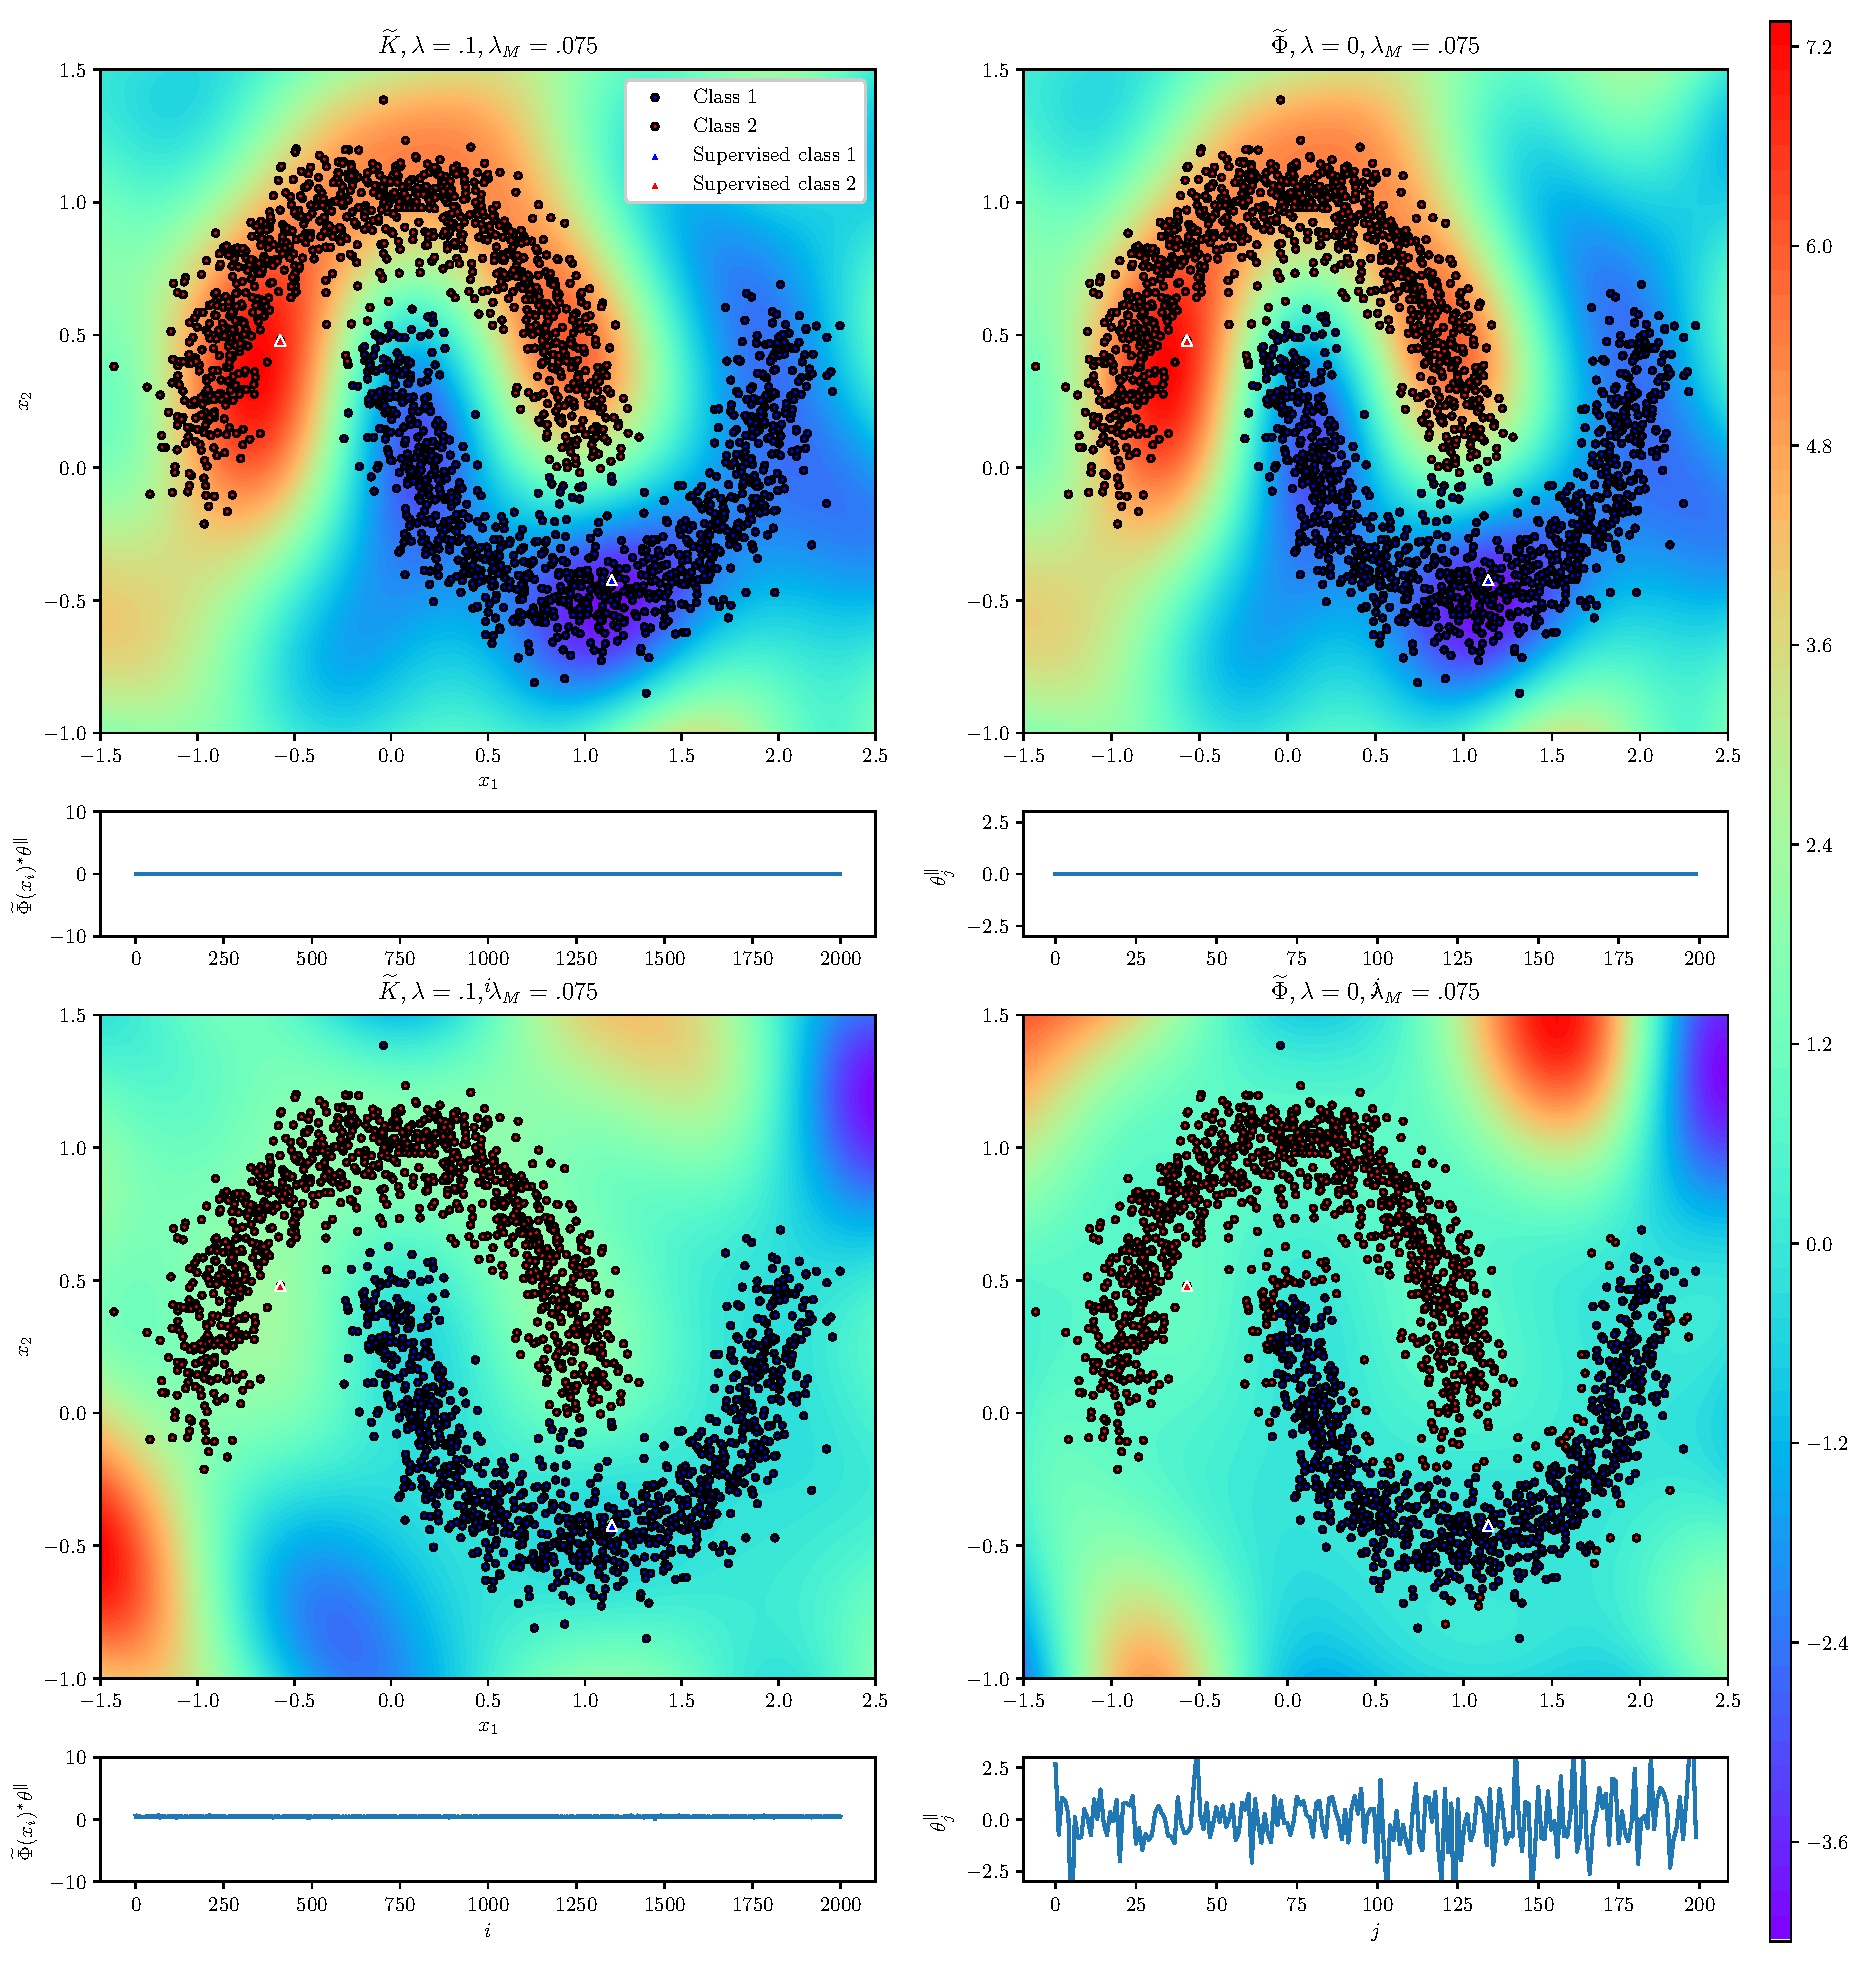
\includegraphics[width=\textwidth]{./gfx/representer_twomoons.eps}
    \caption[\acs{ORFF} equivalence theorem (semi-supervised)]{\acs{ORFF}
    equivalence theorem (semi-supervised). Each row compares the scalar
    \acs{ORFF} $\widetilde{\Phi}$ method constructed from a Gaussian with the
    kernel method where $\widetilde{K}=\widetilde{\Phi}^\transpose
    \widetilde{\Phi}$.  The top row corresponds to the case $\lambda_K=0.1$ and
    $\lambda_M=0.075$.  Since $\lambda_K > 0$, the solution with
    $\widetilde{K}$ and $\widetilde{\Phi}$ are exactly the same
    (\cref{th:orff_representer_semi} applies) and we see that
    $\theta^\parallel=0$. The bottom row corresponds to the case $\lambda_K=0$
    and $\lambda_M=0.075$. Here the solution with $\widetilde{K}$ and
    $\widetilde{\Phi}$ doesn't match (\cref{th:orff_representer_semi} fails to
    apply since $\lambda_K=0$).  Moreover we can see that $\theta^\parallel
    \neq 0$ and $\tildePhi{\omega}(x)^\adjoint \theta \neq 0$, thus $\theta$
    is not in $(\Ker W)^\perp$. \label{fig:representer_semi}}
\end{figure}

\subsection{Gradients}
By linearity and applying the chaine rule to \cref{eq:argmin_theta_semi} and
since $M_{ik}^\adjoint = M_{ki}$ for all $i$, $k\in\mathbb{N}^*_{N+U}$, we have
\begin{dgroup*}
    \begin{dmath*}
        \nabla_{\theta}c\left(V\tildePhi{\omega}(x_i)^\adjoint \theta,
        y_i\right)= \tildePhi{\omega}(x_i)V^\adjoint
        \left(\lderivativeat{c\left(y,
        y_i\right)}{y}{V\tildePhi{\omega}(x_i)^\adjoint
        \theta}\right)^\adjoint,
    \end{dmath*}
    \begin{dmath*}
        \nabla_{\theta}\inner*{\tildePhi{\omega}(x_i)^\adjoint \theta,
        M_{ik}\tildePhi{\omega}(x_k)^\adjoint \theta}_{\mathcal{U}} =
        \tildePhi{\omega}(x_i)\left(M_{ik}+M_{ki}^*\right)
        \tildePhi{\omega}(x_k)^\adjoint \theta,
    \end{dmath*}
    \begin{dmath*}
        \nabla_{\theta}\norm{\theta}^2_{\tildeH{\omega}}=2\theta.
    \end{dmath*}
\end{dgroup*}
Provided that $c(y,y_i)$ is Frechet differentiable \acs{wrt}~$y$, for all $y$
and $y_i\in\mathcal{Y}$ we have $\nabla_{\theta} J_{\lambda_K}(\theta) \in
\tildeH{\omega}$ and
\begin{dmath*}
    \nabla_{\theta} J_{\lambda_K}(\theta) = \frac{1}{N}\sum_{i=1}^N
    \tildePhi{\omega}(x_i)V^\adjoint \left(\lderivativeat{c\left(y,
    y_i\right)}{y}{V\tildePhi{\omega}(x_i)^\adjoint \theta}\right)^\adjoint +
    \lambda_K\theta + \lambda_M\sum_{i,k=1}^{N+U} \tildePhi{\omega}(x_i)M_{ik}
    \tildePhi{\omega}(x_k)^\adjoint \theta
\end{dmath*}
Therefore after factorization, considering $\lambda_K > 0$,
\begin{dmath*}
    \nabla_{\theta} J_{\lambda_K}(\theta)
    = \frac{1}{N}\sum_{i=1}^N \tildePhi{\omega}(x_i)V^\adjoint
    \left(\lderivativeat{c\left(y,
    y_i\right)}{y}{V\tildePhi{\omega}(x_i)^\adjoint \theta}\right)^\adjoint +
    \lambda_K\left(I_{\tildeH{\omega}} + \frac{\lambda_M}{\lambda_K}
    \sum_{i,k=1}^{N+U} \tildePhi{\omega}(x_i)M_{ik}
    \tildePhi{\omega}(x_k)^\adjoint \right)\theta
\end{dmath*}
We note the quantity
\begin{dmath}
    \widetilde{\mathbf{M}}_{\left(\lambda_K,\lambda_M\right)}
    = I_{\tildeH{\omega}} + \frac{\lambda_M}{\lambda_K}\sum_{i,k=1}^{N+U}
    \tildePhi{\omega}(x_i) M_{ik} \tildePhi{\omega}(x_k)^\adjoint \hiderel{\in}
    \mathcal{L}(\tildeH{\omega})
\end{dmath}
so that
\begin{dmath}
    \label{eq:grad_final_semi}
    \nabla_{\theta} J_{\lambda_K}(\theta)
    = \frac{1}{N}\sum_{i=1}^N \tildePhi{\omega}(x_i)V^\adjoint
    \left(\lderivativeat{c\left(y,
    y_i\right)}{y}{V\tildePhi{\omega}(x_i)^\adjoint \theta}\right)^\adjoint +
    \lambda_K\widetilde{\mathbf{M}}_{\left(\lambda_K,\lambda_M\right)}\theta
\end{dmath}
\begin{example}[Naive closed form for the squared error cost]
    Consider the cost function defined for all $y$, $y'\in\mathcal{Y}$ by
    $c(y,y')=\frac{1}{2}\norm{y-y}_{\mathcal{Y}}^2$. Then
    \begin{dmath*}
        \left(\lderivativeat{c\left(y,
        y_i\right)}{y}{V\tildePhi{\omega}(x_i)^\adjoint \theta}\right)^\adjoint
        = \left(V\tildePhi{\omega}(x_i)^\adjoint \theta-y_i\right).
    \end{dmath*}
    Thus, since the optimal solution $\theta_{\seq{z}}$ verifies
    $\nabla_{\theta_{\seq{z}}} J_{\lambda_K}(\theta_{\seq{z}}) = 0$ we have
    \begin{dmath*}
        \frac{1}{N}\sum_{i=1}^N
        \tildePhi{\omega}(x_i)V^\adjoint\left(V\tildePhi{\omega}(x_i)^\adjoint
        \theta_{\seq{z}}-y_i\right) + \lambda_K
        \widetilde{\mathbf{M}}_{\left(\lambda_K,\lambda_M\right)}
        \theta_{\seq{z}}= 0.
    \end{dmath*}
    Therefore,
    \begin{dmath}
        \label{eq:iff_solution_semi} \left(\frac{1}{N}\sum_{i=1}^N
        \tildePhi{\omega}(x_i)V^\adjoint V \tildePhi{\omega}(x_i)^\adjoint +
        \lambda_K \widetilde{\mathbf{M}}_{\left(\lambda_K,
        \lambda_M\right)}\right) \theta_{\seq{z}}
        = \frac{1}{N}\sum_{i=1}^N \tildePhi{\omega}(x_i)V^\adjoint y_i.
    \end{dmath}
    Suppose that $\mathcal{Y}\subseteq\mathbb{R}^p$,
    $V:\mathcal{U}\to\mathcal{Y}$ where $\mathcal{U}\subseteq\mathbb{R}^u$ and
    for all $x\in\mathcal{X}$, $\tildePhi{\omega}(x):
    \mathbb{R}^{r}\to\mathbb{R}^u$ where all spaces are endowed with the
    euclidean inner product. From this we can derive \cref{alg:close_form_semi}
    which returns the closed form solution of \cref{eq:cost_functional} for
    $c(y,y')=\frac{1}{2}\norm{y-y'}_2^2$.
\end{example}
\afterpage{%
\begin{center}
    \begin{algorithm2e}[H]
        \label{alg:close_form_semi}
        \SetAlgoLined
        \Input{\begin{itemize}
            \item $\seq{s}=(x_i,
            y_i)_{i=1}^N\in\left(\mathcal{X}\times\mathbb{R}^p\right)^N$ a
            sequence of supervised training points,
            \item $\seq{u}=(x_i)_{i=N+1}^{N+U}\in\mathcal{X}^{U}$ a sequence of
            unsupervised training points,
            \item $\tildePhi{\omega}(x_i) \in \mathcal{L}\left(\mathbb{R}^u,
            \mathbb{R}^{r}\right)$ a feature map defined for all
            $x_i\in\mathcal{X}$,
            \item $(M_{ik})_{i,k=1}^{N+U}$ a sequence of data dependent
            operators (see \cref{th:orff_representer_semi}),
            \item $V \in \mathcal{L}\left(\mathbb{R}^u, \mathbb{R}^p\right)$ a
            combination operator, \item $\lambda_K \in\mathbb{R}_{>0}$ the
            Tychonov regularization term,
            \item $\lambda_M \in\mathbb{R}_+$ the manifold regularization term.
        \end{itemize}}
        \Output{A model %
        \begin{dmath*} %
            h:\begin{cases} \mathcal{X} \to \mathbb{R}^p \\
            x\mapsto\tildePhi{\omega}(x)^\transpose
            \theta_{\seq{z}},\end{cases} %
        \end{dmath*} %
        such that $\theta_{\seq{z}}$ minimize \cref{eq:cost_functional}, where
        $c(y,y')=\norm{y-y'}_2^2$ and $\mathbb{R}^u$, $\mathbb{R}^r$ and
        $\mathbb{R}^p$ are Hilbert spaces endowed with the euclidean inner
        product.}
        $\mathbf{P} \gets \frac{1}{N}\sum_{i=1}^N
        \tildePhi{\omega}(x_i)V^\transpose  V\tildePhi{\omega}(x_i)^\transpose
        \in\mathcal{L}(\mathbb{R}^{r}, \mathbb{R}^{r})  $\;
        \uIf{$\lambda_M = 0$}{%
            $\widetilde{\mathbf{M}}_{\left(\lambda_K,\lambda_M\right)} \gets
            I_{r} \in\mathcal{L}(\mathbb{R}^{r}, \mathbb{R}^{r})$\;
        }
        \Else{%
            $\widetilde{\mathbf{M}}_{\left(\lambda_K,\lambda_M\right)} \gets
            \left(I_{r} +
            \frac{\lambda_M}{\lambda_K} \sum_{i,k=1}^{N+U}
            \tildePhi{\omega}(x_i) M_{ik} \tildePhi{\omega}(x_k)^\transpose
            \right) \in\mathcal{L}(\mathbb{R}^{r}, \mathbb{R}^{r}) $\;
        }
        $\mathbf{Y} \gets \frac{1}{N}\sum_{i=1}^N
        \tildePhi{\omega}(x_i)V^\transpose  y_i \in \mathbb{R}^{r} $\;
        $\theta_{\seq{z}} \gets \text{solve}_{\theta}\left(\left(\mathbf{P} +
        \lambda_K\widetilde{\mathbf{M}}_{\left(\lambda_K,
        \lambda_M\right)}\right)\theta = \mathbf{Y}\right) \in \mathbb{R}^{r}
        $\;
        \Return $h: x \mapsto \tildePhi{\omega}(x)^\transpose
        \theta_{\seq{z}}$\;
        \caption{Naive closed form for the squared error cost.}
    \end{algorithm2e}
\end{center}}
\begin{figure}
    \centering
    %\resizebox{\textwidth}{!}{\input{./gfx/representer_twomoons.eps}}
    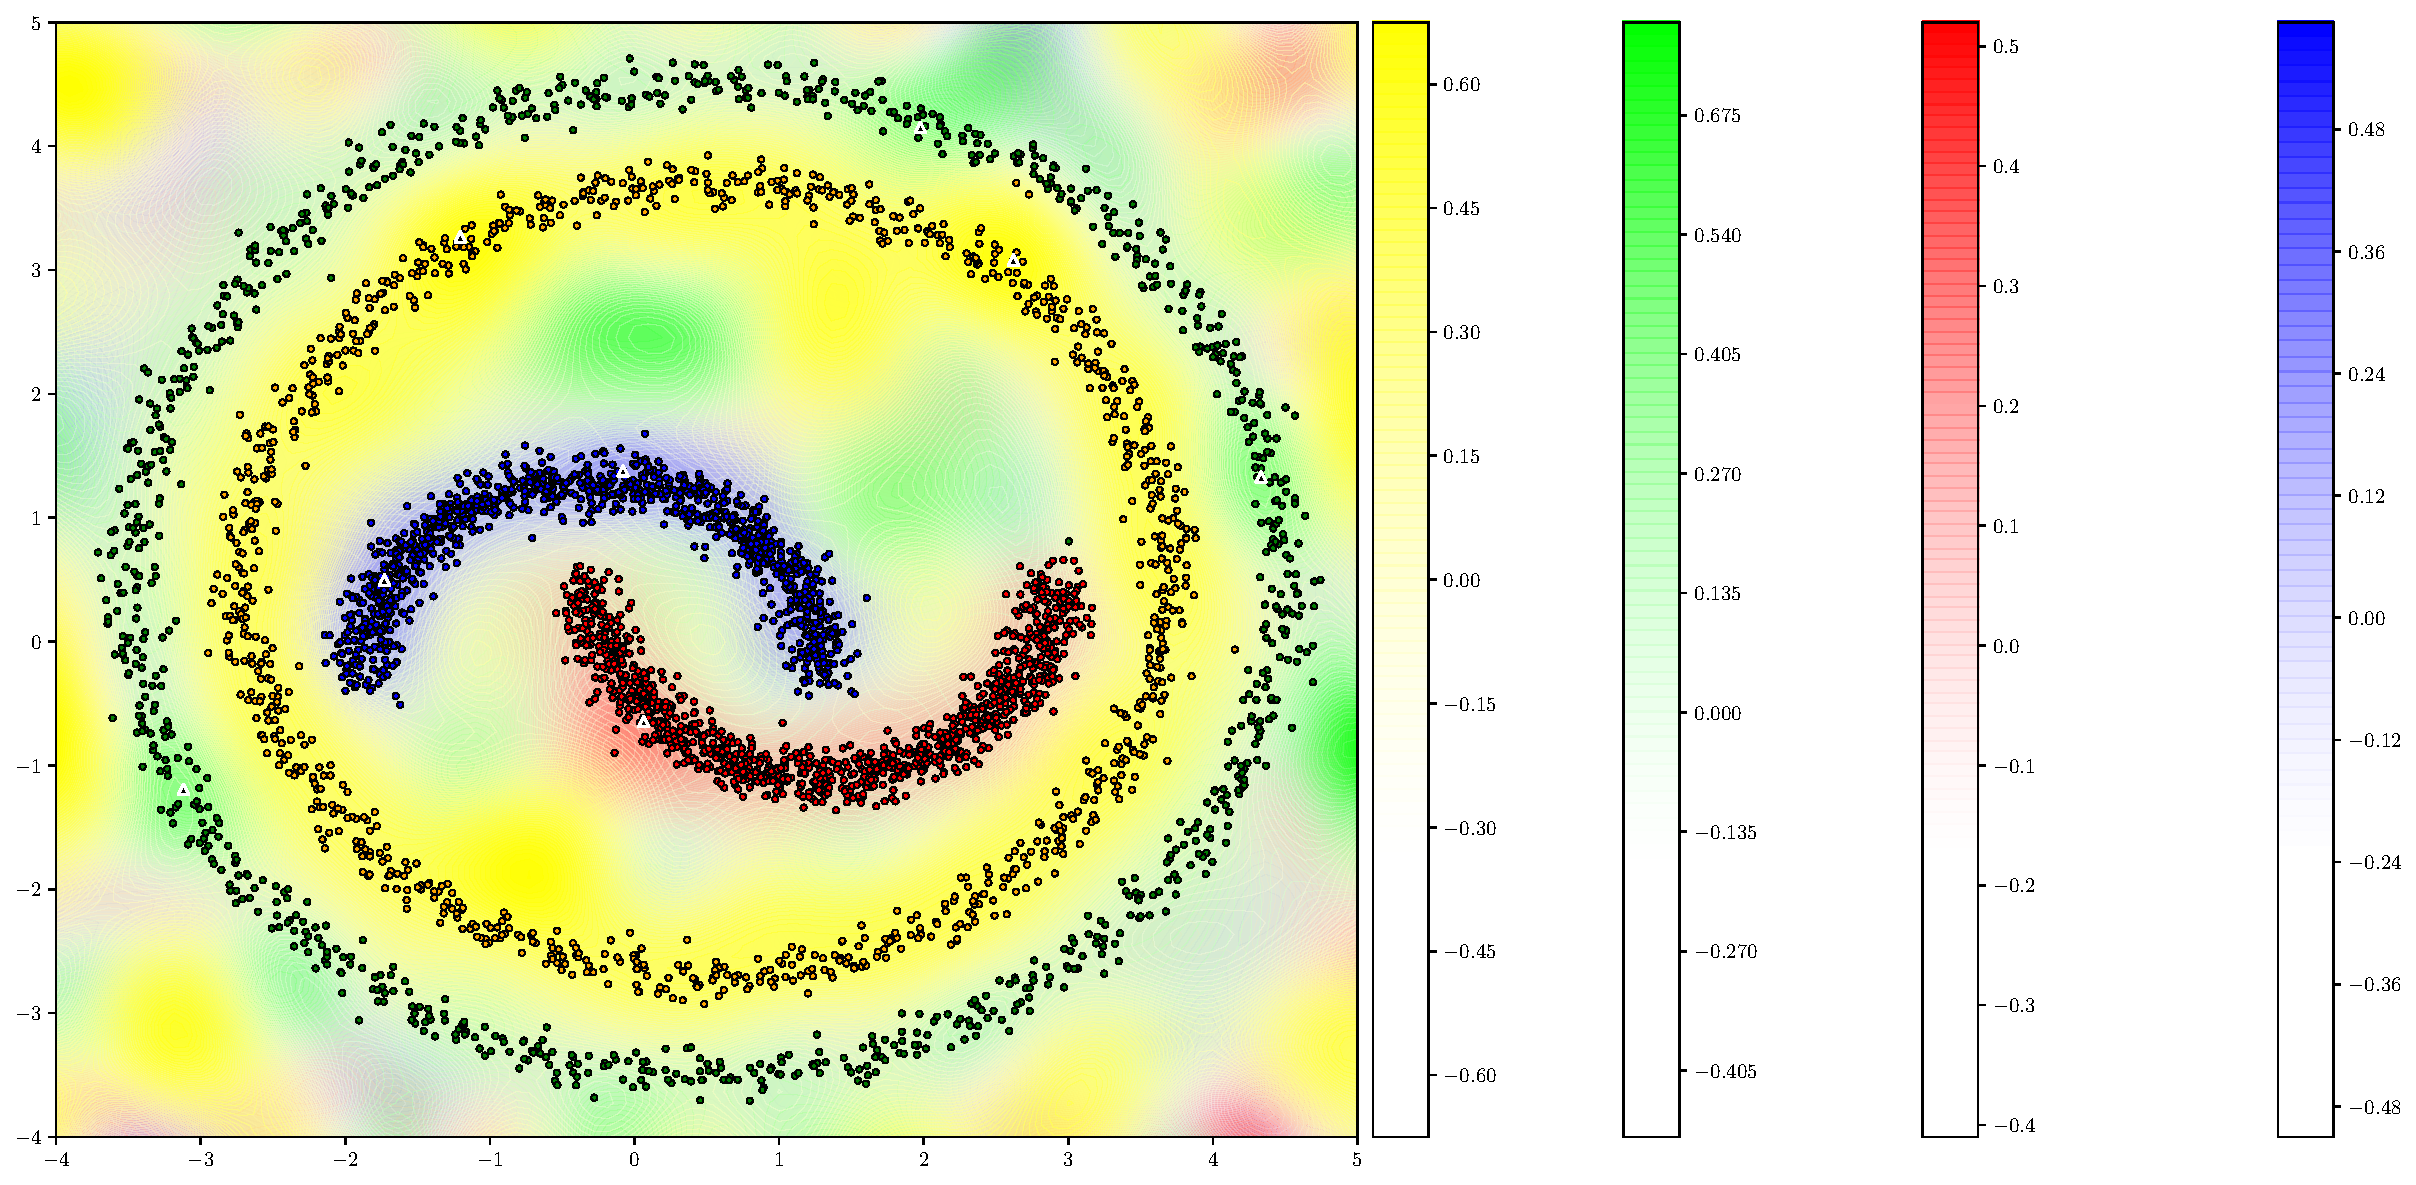
\includegraphics[width=\textwidth]{./gfx/nestedtwomoons.pdf}
    \caption[\acs{ORFF} multiclass semi-supervised]{Semi-supervised learning
    on a multiclass nested circle and two moons dataset. We performed an 
    unsupervised spectral clustering \citep{von2007tutorial} step to construc
    the matrices $M_{ik}$'s and, choose the matrix $B$ of the \acs{ORFF} using
    the simplex coding \citep{mroueh2012multiclass}.}
\end{figure}
\subsection{Complexity}
Suppose that $u=\dim(\mathcal{U})<+\infty$ and
$u'=\dim(\mathcal{U}')<\infty$ and for all $x\in\mathcal{X}$,
$\tildePhi{\omega}(x):\mathcal{U}'\to\tildeH{\omega}$ where
$r=\dim(\tildeH{\omega})<\infty$ is the dimension of the redescription space
$\tildeH{\omega}=\mathbb{R}^{r}$. Since $u$, $u'$, and $r<\infty$, we view the
operators $\tildePhi{\omega}(x)$, $V$ and
$\widetilde{\mathbf{M}}_{\left(\lambda_K,\lambda_M\right)}$ as matrices.
Computing $V^\adjoint V$ cost $O_t(u^2p)$. Step 1 costs $O_t(r^2u + ru^2)$.
Steps 5 (optional) has the same cost except that the sum is done over all pair
of $N+U$ points thus it costs $O_t((N+U)^2(r^2u + r u^2))$. Steps 7 costs
$O_t(N(ru + up))$. For step 8, the naive inversion of the operator costs
$O_t(r^3)$. Eventually the overall complexity of \cref{alg:close_form_semi} is
\begin{dmath*}
    O_t\left(ru(r + u) \begin{cases} (N+U)^2 & \text{if $\lambda_M > 0$} \\ N &
    \text{if $\lambda_M = 0$} \end{cases}+ r^3 + Nu(r+p) \right),
\end{dmath*}
while the space complexity is $O_s(r^2)$. This complexity is to compare with
the kernelized solution proposed by~\citet{minh2016unifying}. Let
\begin{dmath*}
    \mathbf{K}:
    \begin{cases}
        \mathcal{U}^{N+U} \to \mathcal{U}^{N+U} \\
        u\mapsto\Vect_{i=1}^{N+U}\sum_{j=1}^{N+U}K(x_i, x_j)u_j
    \end{cases}
\end{dmath*}
and
\begin{dmath*}
    \mathbf{M}:
    \begin{cases}
        \mathcal{U}^{N+U} \to \mathcal{U}^{N+U} \\
        u\mapsto\Vect_{i=1}^{N+U}\sum_{k=1}^{N+U}M_{ik}u_k.
    \end{cases}
\end{dmath*}
When $\mathcal{U}=\mathbb{R}$,
\begin{dmath*}
    \mathbf{K}=
    \begin{pmatrix} K(x_1, x_1) & \hdots & K(x_1, x_{N+U}) \\ \vdots
        & \ddots & \vdots \\  K(x_{N+U}, x_1) & \hdots & K(x_{N+U}, x_{N+U})
    \end{pmatrix}
\end{dmath*}
is called the Gram matrix of $K$. When $\mathcal{U}=\mathbb{R}^p$, $\mathbf{K}$
is a matrix-valued Gram matrix of size $u(N+U)\times u(N+U)$ where each entry
$\mathbf{K}_{ij}\in\mathcal{M}_{u,u}(\mathbb{R})$. When
$\mathcal{U}=\mathbb{R}^u$, $\mathbf{M}$ can also be seen as a matrix-valued
matrix where each entry is $M_{ik}\in\mathcal{M}_{u,u}(\mathbb{R})$. We also
introduce the matrices $\mathbf{V}^\transpose  \mathbf{V}\colonequals I_{N+U}
\otimes (V^\transpose  V)$ and
\begin{dmath*}
    \mathbf{P}:
    \begin{cases}
        \mathcal{U}^{N+U} \to \mathcal{U}^{N+U} \\ u\mapsto
        \left(\Vect_{j=1}^Nu_j\right) \oplus \left(\Vect_{j=N+1}^{N+U}0\right)
    \end{cases}
\end{dmath*}
The operator $\mathbf{P}$ is a projection that sets all the terms $u_j$, $N < j
\le N + U$ of $u$ to zero. When $\mathcal{U}=\mathbb{R}^u$ it can also be seen
as the block matrix of size $u(N+U) \times u(N + U)$ and
\begin{dmath*}
    \mathbf{P}=
    \begin{pmatrix}
        & & & 0 & \hdots & 0 \\ & I_u \otimes I_{N} & & \vdots & \ddots &
        \vdots \\ & & & 0 & \hdots & 0 \\ 0 & \hdots & 0 & 0 & \hdots & 0 \\
        \vdots & \ddots & \vdots & \vdots & \ddots & \vdots \\ 0 & \hdots & 0 &
        0 & \hdots & 0
    \end{pmatrix}
\end{dmath*}
Then the equivalent kernelized solution $u_{\seq{z}}$ of
\cref{th:representer_semi} is given by~\citet{minh2016unifying}
\begin{dmath*}
    \left(\frac{1}{N}\mathbf{V}^\transpose  \mathbf{V} \mathbf{P} \mathbf{K} +
    \lambda_M \mathbf{M} \mathbf{K} + \lambda_K
    I_{\Vect_{i=1}^{N+U}\mathcal{U}}\right)u_{\seq{z}}=\left(\Vect_{i=1}^N
    V^\transpose  y_i\right) \oplus \left(\Vect_{i=N+1}^{N+U} 0 \right).
    \end{dmath*}
which has time complexity $O_t(((N+U)u)^3+ Nup)$ and space complexity
$O_s(((N+U)u)^2)$. Notice that computing the
data dependent norm (manifold regularization) is expensive. Indeed when
$\lambda_M=0$, \cref{alg:close_form_semi} has a linear complexity with respect
to the number of supervised training points $N$ while the complexity becomes
quadratic in the number of supervised and unsupervised training points $N+U$
when $\lambda_M>0$.
